\documentclass[a4paper,11pt]{article}

\usepackage[utf8]{inputenc} % allow utf-8 input
\usepackage{hyperref}       % hyperlinks
\usepackage{url}            % simple URL typesetting
\usepackage{booktabs}       % professional-quality tables
\usepackage{amsfonts}       % blackboard math symbols
\usepackage{nicefrac}       % compact symbols for 1/2, etc.
\usepackage{microtype}      % microtypography
\usepackage{graphicx}       % include graphics
\usepackage{subcaption}     % subfigures
\usepackage{float}          % placement of floats
\usepackage{fancyhdr}       % head notes and foot notes
\usepackage{bbm}            % Nice symbols
\usepackage{mathtools}      % Math tools like operators
\usepackage{algorithm}      % For writing algorithm
\usepackage[noend]{algpseudocode} % For writing pseudocode
\graphicspath{ {images/} }



\newcommand{\RR}{\mathbbm{R}} % Nice R sign
\DeclarePairedDelimiter\abs{\lvert}{\rvert} % abs
\DeclarePairedDelimiter\norm{\lVert}{\rVert} % norm
\DeclareMathOperator*{\argmin}{arg\,min} % argmin
\DeclareMathOperator*{\argmax}{arg\,max} % argmax

\title{P3 - Dictionary learning, application to denoising and inpainting}


\author{
  Louis Martin\\
  \href{mailto:louis.martin@student.ecp.fr}{\tt louis.martin@student.ecp.fr}
}

\pagestyle{fancy}
\fancyhf{}
\lhead{Louis MARTIN}
\rhead{Sparsity and Compressed Sensing: Project}

\rfoot{Page \thepage}

\begin{document}

\maketitle

\begin{abstract}
%% Abstract (½ page):
%% What problem(s) is studied ?
This paper will focus on how to efficiently learn a dictionary in order to obtain a sparse representation of a signal (e.g. image or audio).
%% Why is it relevant ?
Deriving a sparse representation of a signal can be very efficient in solving multiple signal processing problems.
It has been successfully used in compression, inpainting, denoising, inverse problems and more.
One way to obtain a sparse coding is by using dictionaries.
A dictionary acts as a basis on which the data can be accurately represented using a small number of coefficients.
This basis can be either predefined or learned, both approaches have shown great results.
We will here focus how to efficiently learn an appropriate dictionary given the data we want to encode.
Finding a good dictionary is indeed important because it will define the representational power of the sparse coding,
i.e. how well the sparse coded signal will represent the original signal.
The learning process is therefore a key step for sparse representation.
% TODO:
%% What solution(s) is proposed ?
We propose to study and conpare three different approaches to dictionary learning.
An intuitive block coordinate gradient descent
%% Which contributions (theory, numerics, etc) ?

\end{abstract}

\section{Introduction}
%% Introduction (~3 pages) :
%% Presentation of the problem(s).
Sparse coding is able to solve multiple signal processing tasks such as compression, inpainting, denoising, texture synthesis and so on.
% Why do we want sparsity, i.e. a small number of non-zero coefficients ?
% 1) Compression
Sparsity, i.e. having a small number of non-zero coefficients, is wanted for several of its useful properties.

It is very effective for compression for obvious reasons of storage space, we only have to store a small set of sparse coefficients that will permit an accurate reconstruction if the original signal.
% 2) Theorem in the first lecture -> good compression coefficients => good denoising

Good compression coefficients also often implies good denoising properties.
Noise is indeed often small local high frequency and unstructured information that is pruned by the sparse coding.
% 3) Natural images tend to have a small number of non-zero coefficients.
% Complex images like random images (or lot of noise) or trees will have a higher number of coefficient.
Natural image tend to have a small number of non-zero coefficient whereas complex images like random images or images with trees will have a higher number of coefficients.
% Sparsity is the a good indicator of natural images
Sparsity is therefore a good indicator of natural images.

%% Previous works (at least a few citations). If relevant, include things that you have seen during the MVA course (or possibly other courses).
The choice of the space in which the sparse representation lives is important.
The problem is often reduced to finding a good basis for this space.
It can be either be predefined or learned.

One can use a predefined basis which will be fixed for all tasks and datasets such as the Fourier basis or the wavelet basis thanks to \cite{mallat99}.
The fact that such a basis does not depend on the data makes it hard to design but also powerful because it can be reused for and define a standard.
The good sparse representation of natural images in the wavelet space led to the success of the JPEG2000 algorithm for image compression, see \cite{marcellin00}.

Another approach is to learn the basis, which is what we will focus on in this paper.
From this point on we will interpret this basis as a dictionary for reasons that we will explain later.
A dictionary is a set of representative signals called atoms.
The signal of interest is therefore expressed as a linear combination of these atoms.

Having a learned dictionary that is specific to a certain type of data or to one image in particular can be very powerful.
The sparse representation can at the same time be sparser and represent the data better.
Another key idea is to design overcomplete dictionaries which means that there are more atoms than the each atom dimension and so these atoms are not linearly independent.
This is why the term basis to denote an overcomplete dictionary is abusive.
Instead of being harmful, designing overcomplete dicionaries gives more flexibility to the sparse representation and leads to easier problems.
The decomposition is not unique anymore as it would be with orthogonal basis such as Fourier or wavelet.
% TODO:
%% Contributions. Why is the studied method different/better/worse/etc. than existing previous works.
%% TODO: P Stock While this intuitive bag-of-features approach is widely used in computer vision [6


\section{Problem statement}
\subsection{Notations}
Given a signal of size $m$, \textbf{$y \in \RR^m$}, a dictionary is a collection of $k$ prototype signal atoms represented in a matrix $D \in \RR^{m \times p}$
We want to find $x \in \RR^p$, the sparse representation of $y$ in the dictionary $D$.
We want an exact representation $D x = y$ or more frequently an approximate representation $ D x \approx y$.
A sparse vector is a vector with a "small" number of non-zero coefficient.
The sparsity measure is the $l_0$ pseudo-norm denoted $\norm{.}_0$.
The sparsity constraint then writes $\norm{x}_0<k$ with $k \in \mathbbm{N}$.

The problem we want to solve is therefore
$$\min\limits_{D \in \RR^{m \times p}, x \in \RR^p} \norm{y - Dx}_2^2  \text{  subject to  } \norm{x}_0<k$$


The sparsity measure, the $l_0$ pseudo-norm is non-convex which makes the problem hard to solve in many approaches like gradient descent because we are not guaranteed to find a minimum.
Given that $\forall p <1$, the $l_p$ pseudo-norm is non convex, the closest convex norm that we can use is the $l_1$ norm which is in practice a good measure of the sparsity of a signal compared to other norms.
This norm favors sparse representation as can be seen in figure \ref{l1l2_norm}

\begin{figure}[!htbp]
\centering
  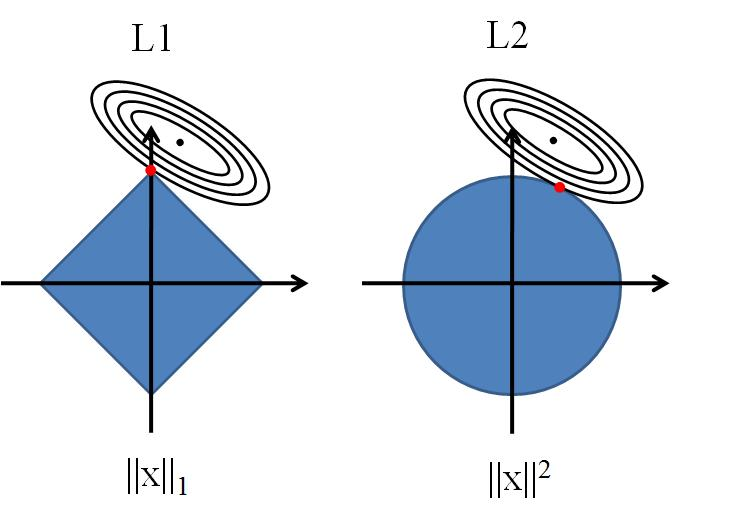
\includegraphics[width=0.5\linewidth]{l1l2_norm.jpg}
  \caption{The $l_1$ norm favors sparisty}
  \label{l1l2_norm}
\end{figure}

The constraint on $x$ will be traduced by $\chi_k = \{ x \in \RR^{p \times n}, \norm{x}_0<k \}$.
Furthermore we will want the dictionary to have normalized atoms.
Otherwise the atoms norm will increase for the sole purpose of decreasing the sparse representation norm and hence the $l_1$ constraint.
To prevent this behaviour from occuring we  will want $ D \in \mathcal{D} $ with $\mathcal{D} = \{ D \in \RR^{m \times p}, \forall i=1 \ldots p, \norm{D_{\cdot,i}} \leq 1 \}$.

We will often want to minimize the error over $n$ signals which will give us
$$\min\limits_{D \in \mathcal{D}, (x_i)_{i=1}^n \in \chi_k} \sum\limits_{i=1}^n \norm{y_i - Dx_i}_2^2$$
with $Y \in \RR^{m \times n}, Y = [y_1 \ldots y_n]$ and $X \in \RR^{p \times n}, X = [x_1 \ldots x_n]$.

The problem now rewrites:
\begin{equation} \label{eq:1}
\min\limits_{D \in \mathcal{D}, X \in \chi_k} E(X,D) = \min\limits_{D \in \mathcal{D}, X \in \chi_k} \norm{Y - DX}_F^2
\end{equation}

In order to use proximal methods we can also rewrite \label{eq:1} by:
$$\min E(X,D) + \iota_{\chi_k}(X) + \iota_{\mathcal{D}}(D)$$
with $\iota_C$ the indicator of $C$ defined by
$ \iota_C(x) =
\begin{cases}
0, & \text{if } x \in C\\
+ \infty, & \text{otherwise}
\end{cases}
$

\subsection{Splitting the dictionary learning task into two subproblems}
Minimizing \ref{eq:1} both over $D$ and $X$ jointly is often not feasible.
That is why many approach split it into two subproblems that can be solved iteratively.
The first is to sparse code the data given the dictionary and the second to update the dictionary given this sparse coding.

% TODO:
 A natural approach to solving
this problem is to alternate between the two variables, minimizing over one while keeping the other
one fixed, as proposed by Lee et al. (2007) (see also Engan et al. 1999 and Aharon et al. 2006, who
use $l_0$ rather than $l_1$ penalties, or Zou et al. 2006 for the problem of sparse principal component
analysis).4

\subsubsection{Finding the sparse representation}
This subproblem writes:
\begin{equation} \label{eq:2}
X \in \argmin_{X \in \chi_k} \norm{Y - DX}^2
\end{equation}
Equation \ref{eq:2} is typically solved by iterating over X until we have a solution that yields a small enough error $E(X,D)$.

There is a whole range of pursuit algorithms that use this approach.

Matching pursuit was introduced by \cite{mallat93} and successfully applied to signal decomposition.
The algorithm finds for each signal $y$, the atom $d_i$ which captures the most energy in the sense that
$$d_i = \argmax_{d_i \in D} |<y, d_i>|$$.
The corresponding coefficient is then set to $$x_i = \frac{<y, d_i>}{\norm{d_i}^2}$$ and the captured information is removed from $y$ so that $$y \leftarrow y - x_i d_i$$.
This process is repeated until we reach the wanted sparsity or until the error is below a specified threshold.

% TODO: (mairal10a)
A number of recent methods for solving this type of problems are based on coordinate
descent with soft thresholding (Fu, 1998; Friedman et al., 2007; Wu and Lange, 2008).

MP OMP FOCUSS \cite{gorodnitsky97} PGD
Wikipedia -> A popular extension of Matching Pursuit (MP) is its orthogonal version: Orthogonal Matching Pursuit[11][12] (OMP). The main difference from MP is that after every step, all the coefficients extracted so far are updated, by computing the orthogonal projection of the signal onto the set of atoms selected so far. This can lead to better results than standard MP, but requires more computation.
\subsubsection{Finding the dictionary}
PGD MOD
Finding the best sparse representation of a signal is a NP-Hard problem, that is why we will approximate the signal.
% TODO: citation with author and date
% TODO: talking of 'basis' is abusive because it is often overcomplete
%%%%%%%%%% Taken from \cite{matrixfactorization}
%recently led to state-of-the-art
%results in numerous low-level signal processing tasks such as image denoising (Elad and Aharon,
%2006; Mairal et al., 2008b), texture synthesis (Peyre, 2009) and audio processing (Grosse et al.,
%2007; Fevotte et al., 2009; Zibulevsky and Pearlmutter, 2001), as well as higher- level tasks such as
%image classification (Raina et al., 2007; Mairal et al., 2008a, 2009b; Bradley and Bagnell, 2009;
%Yang et al., 2009),
%%%%%%%%%%
%The learnt basis look like wavelets / Gabor filters but are tuned to the data -> better accuracy
Not penalizing the dictionary -> dictionary values will increase for the sparse coef to tend to 0
\cite{olshausen97} (k-SVD p-4313 [24]).
\section{Dictionary learning methods}
%% Main body (~10 pages) :
%% Presentation of the method(s).
%% Theoretical guarantees.
%% Numerics.
Most of the iterative methods are composed of the two steps defined above.
Sparse coding the vector and updating the dictionary given this sparse representation.


\subsection{Proximal methods}
% TODO:
\cite{olshausen97} (k-SVD p-4313 [24])
% TODO:
In the case of dictionary learning, the classical projected first-order projected stochastic gradient
descent algorithm (as used by Aharon and Elad 2008; Kavukcuoglu et al. 2008 for instance) consists
of a sequence of updates of D:



A intuitive and efficient algorithm for dictionary learning is to use a block coordinate gradient descent approach as in implemented in \cite{nt4} and is shown to converge in \cite{tseng01}.
This algorithm is part of the category of proximal methods and has gained substantial attention in signal processing \cite{combettes11}.
This is a two step algorithm.
We initialize $n$ training signals $(y_i \in \RR^m)_{i=1}^{n}$
that we put in a matrix $Y \in \RR^{m \times n}, Y = [y_1 \ldots y_n]$.
\begin{itemize}
  \item First we find the best sparse representation of the data given a fixed dictionary.
  	\begin{equation} \label{eq:pgd1}
      X^{(i+1)} \in \argmin_{X \in \chi_k} \norm{Y - D^{(i)}X}^2
	\end{equation}
  \item Then we update the dictionary given this sparse representation.
  	\begin{equation} \label{eq:pgd2}
      D^{(i+1)} \in \argmin_{D \in \mathcal{D}} \norm{Y - DX^{(i+1)}}^2
	\end{equation}
\end{itemize}


\subsubsection*{Forward-Backward algorithm}
\ref{eq:pgd1} and \ref{eq:pgd2} can be solved using the Forward-Backward proximal algorithm which is detailed in \cite{combettes11}, \cite{parikh14} and in the class lectures.
We have
\begin{equation*}
\begin{split}
x^* \in \argmin_x F(x) + G(x) & \Longleftrightarrow 0 \in \nabla F(x^*) + \partial G(x^*)\\
							  & \Longleftrightarrow (x^* - \gamma \nabla F(x^*)) \in x^* + \gamma \partial G(x^*)\\
                              & \Longleftrightarrow x^* = Prox_{\gamma G} (x^* - \gamma \nabla F(x^*))
\end{split}
\end{equation*}

The Forward-Backward update thus reads
$$x^{(i+1)} = Prox_{\gamma G} (x^{(i)} - \gamma \nabla F(x^{(i)})$$
with the proximal operator being an natural extension of the projection on a convex set.
$$Prox_{\gamma G}(x) = \argmin_z \frac{1}{2} \norm{x - z}^2 + \gamma G(z)$$

When $G = \iota_C$ then the proximal operator is the projection on the convex set C.
$$Prox_{\gamma G}(x) = \argmin_{z \in C} \norm{x - z} = \Pi_C(x)$$
In this special case, Forward-Back is equivalent to \emph{projected gradient descent}


\subsubsection*{Back to dictionary learning}
\ref{eq:pgd1} and \ref{eq:pgd2} can be rewritten as
$$\argmin_X E(X,D) + \iota_{\chi_k}$$
$$\argmin_D E(X,D) + \iota_{\mathcal{D}}$$

We thus only need compute the gradient of $E(X,D)$ with respect to X and D and apply the Forward-Backward update rule to finally have:

$$ X^{(i+1)} = X^{(i)} - \gamma D^T (D^{(i)}X^{(i)} - Y) $$
$$ D^{(i+1)} = D^{(i)} - \tau (D^{(i)}X^{(i+1)} - Y) X^T $$

\begin{algorithm}
\caption{Projected gradient descent}\label{pgd}
\begin{algorithmic}[1]
\State toto
\end{algorithmic}
\end{algorithm}

\begin{figure}[!htbp]
\centering
  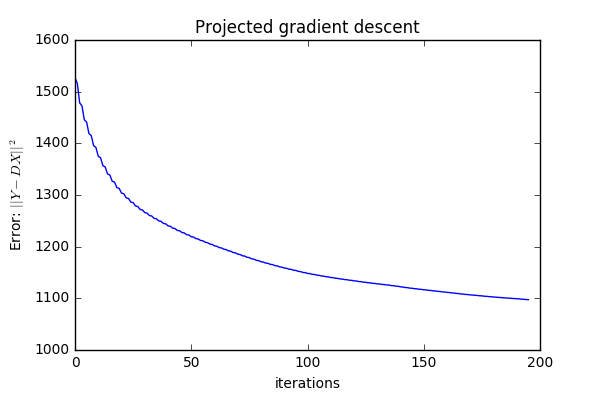
\includegraphics[width=\linewidth]{projected_gradient_descent.png}
\end{figure}0

\subsection{K-SVD}
The approach in \cite{aharon06} is interesting in the way that it considers the dictionary learning problem as a generalization of a clustering problem. Clustering is indeed an extreme case of sparse coding where there is only one non-zero coefficient and this coefficient must be one.

The K-SVD algorithm can be used with any sparse coding technique because it is focused on the dictionary update.
Each column $d_k$ of the dictionary is updated independently takes to a good decomposition of the error $E(X,D)$ into a matrix that does not depend on $d_k$ and a rank 1 matrix that does.
\begin{equation} \label{eq:ksvd1}
\begin{split}
  E(X,D) & = \norm{Y - DX}_F^2 \\
  		 & = \norm{Y - \sum\limits_{j=1}^{p} d_j x^j} \text{ ($x^j$ is the $j$th row, not the column $x_j$)}\\
         & = \norm{(Y - \sum\limits_{j \neq k} d_j x^j)  - d_k x^k}
\end{split}
\end{equation}

We will then subset these matrices to only keep the parts that use the column $d_k$.
That is why the ensemble $\omega_k = \{i | i = 1 \ldots N, x^k(i) \neq 0\}$, is introduced. It denotes the indices of the samples that use the atom $d_k$.
Using this ensemble we can construct the matrix $\Omega_k \in N \times |\omega_k|$ with ones at the $(\omega_k(i),i)$ coordinates and zeros everywhere else.

This matrix will subset the problem to only the values concerned by the update of the column $d_k$.

We can now rewrite the minimization of the error defined in \ref{eq:ksvd1} as
\begin{equation*}
\begin{split}
  \min_{d_k \in \mathcal{D}, x^k \in \chi_k} \norm{E_k - d_k x^k }_F^2 & = \min_{d_k \in \mathcal{D}, x^k \in \chi_k} \norm{E_k \Omega_k - d_k x^k \Omega_k}_F^2 \\
  											& = \min_{d_k \in \mathcal{D}, x^k_R} \norm{E_k^R - d_k x^k_R}_F^2 \\
                                            & \text{ (with $E_k^R$ and $x^k_R$ only values concerned by $d_k$)}
\end{split}
\end{equation*}

Note that we optimize on both $d_k$ and $x^k_R$ at the same time. The restriction of $x^k$ to $x^k_R$ also forces it to have the same support before and after the update so that we don't need to explicitely enforce the sparsity constraint.
This basically boils down to finding the best rank one matrix approximation of $E_k^R$.
With $E_k^R = U \Delta V^T$ being the SVD decomposition of $E_k^R$, Eckart–Young–Mirsky theorem states that $\sigma_1 u_1 v_1^T$ is the best rank one approximation of $E_k^R$.\\
The update rule is therefore $d_k \leftarrow u_1$ and $x^k_R \leftarrow \sigma_1 v_1$.
This step is repeated for all the columns as it is done for the means in K-means thus the name K-SVD.


\subsection{Online learning for matrix factorization}
\cite{mairal10}
\ref{eq:1} can be interpreted as a matrix factorization problem. Indeed we try to find a factorization of $Y$ in the form $DX$.
When confronted with a very large number of samples $N$, it is impractical to work directly with the $Y$ and $X$ matrices. That is why this paper proposes to solve the problem iteratively, sample by sample in an online fashion. Online learning also reduces overfitting if given a big enough dataset.

The method proposed draws random samples as in stochastic gradient descent, derive its sparse representation and then updates the dictionary.
However the objective is to not only update the dictionary based on the current sample but also on all the samples that we previously considered in order to have a more substantial update.
The sparse coding step is done using the $l_1$ penalty with LARS-lasso algorithm from \cite{efron04}.

Let's rewrite the update rule in a form that will lead to an efficient algorithm.
\begin{equation*}
\begin{split}
  D_t & = \argmin_{D \in \mathcal{D}} \frac{1}{t} \sum\limits_{i=1}^t (\frac{1}{2} \norm{y_i - D x_i}_2^2 + \lambda \norm{x_i}_1)\\
      & = \argmin_{D \in \mathcal{D}} \frac{1}{t}  (\frac{1}{2} \norm{Y_t - DX_t}_F^2 + \lambda \norm{X_t}_{1,1})\\
      & = \argmin_{D \in \mathcal{D}} \frac{1}{t}  (\frac{1}{2} \norm{Y_t - DX_t}_F^2) \text{   ($\norm{X_t}_{1,1}$ does not depend on $D$)}\\
      & = \argmin_{D \in \mathcal{D}} \frac{1}{t}  (\frac{1}{2} Tr((Y_t - DX_t)^T (Y_t - DX_t)))\\
      & = \argmin_{D \in \mathcal{D}} \frac{1}{t}  (\frac{1}{2} Tr(Y_t Y_t^T) - Tr(X_t^T D^T Y_t) + \frac{1}{2} Tr(X_t^T D^T D X_t))\\
      & = \argmin_{D \in \mathcal{D}} \frac{1}{t}  (\frac{1}{2} Tr(D^T D X_t X_t^T) - Tr(D^T Y_t X_t^T) )\\
      & = \argmin_{D \in \mathcal{D}} \frac{1}{t}  (\frac{1}{2} Tr(D^T D A_t) - Tr(D^T B_t) )
\end{split}
\end{equation*}

We can decompose $A_t$ and $B_t$ as follows:
$$ A_t = \sum\limits_{i=1}^t x_i x_i^T \text{ and } B_t = \sum\limits_{i=1}^t y_i x_i^T $$
We can therefore update $A_t$ and $B_t$ for each sample and not compute them from scratch every time.

We can then update each column independently with:
$$ u_j \leftarrow \frac{1}{A[j,j](b_j - D a_j) + d_j} $$
$$ d_j \leftarrow \frac{1}{\max(\norm{u_j}_2, 1)} u_j $$

% TODO:
This algorithm is shown to converge to a solution $D^*$ and note that it does not depend on any paramater such as a learning rate.

\section{Conclusion}
%% Conclusion and perspective (~1 page)
%% Summary of the result obtained: pros and cons (limitation, problems, error in the articles, etc)
%% Possible improvement/extension
First filters of neural networks -> looks like a dictionary



\begin{thebibliography}{9}
%% Bibliography (~1 page)
\bibitem{mairal10}
  J. Mairal, F. Bach, J.Ponce, G. Sapiro,
  \emph{Online Learning for Matrix Factorization and Sparse Coding},
  Journal of Machine Learning Research 11 19-60, 2010.
  % http://www.di.ens.fr/~fbach/mairal10a.pdf

\bibitem{aharon06}
  Aharon, Michal, Michael Elad, and Alfred Bruckstein. "K-SVD: An Algorithm for Designing Overcomplete Dictionaries for Sparse Representation." IEEE Transactions on signal processing 54.11 (2006): 4311-4322.

 %TODO: beautify
\bibitem{mallat99}
. Mallat. A Wavelet Tour of Signal Processing, Second Edition. Academic Press, New York,
September 1999.

\bibitem{mallat93}
%http://www.cmap.polytechnique.fr/~mallat/papiers/MallatPursuit93.pdf

\bibitem{marcellin00}
M. W. Marcellin, M. J. Gormish, A. Bilgin, and M. P. Boliek, “An
overview of JPEG-2000,” in Proc. Data Compression Conf., 2000, pp.
523–541.

\bibitem{olshausen97}
B. A. Olshausen and B. J. Field, “Sparse coding with an overcomplete
basis set: A strategy employed by v1?,” Vision Res., vol. 37, pp.
3311–3325, 1997.

\bibitem{gorodnitsky97}
% http://citeseerx.ist.psu.edu/viewdoc/download?doi=10.1.1.154.6856&rep=rep1&type=pdf

\bibitem{nt4}
%https://github.com/gpeyre/numerical-tours/blob/master/matlab/sparsity_4_dictionary_learning.ipynb

\bibitem{tseng01}
P. Tseng, , J. Optim. Theory Appl., 109, 2001, 475-494.

\bibitem{parikh14}
Proximal Algorithms.
N Parikh, SP Boyd - Foundations and Trends in optimization, 2014 - web.stanford.edu

\bibitem{efron04}
Efron, Bradley, et al. "Least angle regression." The Annals of statistics 32.2 (2004): 407-499.

\bibitem{combettes11}
Combettes, Patrick L., and Jean-Christophe Pesquet. "Proximal splitting methods in signal processing." Fixed-point algorithms for inverse problems in science and engineering. Springer New York, 2011. 185-212.

\end{thebibliography}
\end{document}
% Information for the project report:
% If possible, write the report in english.
% You must bring a printed version with your to give me before the presentation. This is a strict deadline.
% Using Latex is highly recommended.
% Roughly 15 pages (A4, 11pt font, single column), including roughly one page of bibliography.
% Should be similar to a (short) scientific article in an applied mathematics journal.
% No source code.
% When presenting the numerics, give all parameters, so that the results are reproducible.
% It should not be a rewriting of the original article. You should only report about what you have done, and only explain the theory that is relevant to explain the numerics you have done.
% Suggestion of structure for the report:
% Abstract (½ page):
% What problem(s) is studied ?
% Why is it relevant ?
% What solution(s) is proposed ?
% Which contributions (theory, numerics, etc) ?
% Introduction (~3 pages) :
% Presentation of the problem(s).
% Previous works (at least a few citations). If relevant, include things that you have seen during the MVA course (or possibly other courses).
% Contributions. Why is the studied method different/better/worse/etc. than existing previous works.
% Main body (~10 pages) :
% Presentation of the method(s).
% Theoretical guarantees.
% Numerics.
% Conclusion and perspective (~1 page)
% Summary of the result obtained: pros and cons (limitation, problems, error in the articles, etc)
% Possible improvement/extension
% Bibliography (~1 page)
%
%
% P3 - Dictionary learning, application to denoising and inpainting
% [Louis MARTIN]
% http://www.numerical-tours.com/matlab/sparsity_4_dictionary_learning/
% http://www.numerical-tours.com/matlab/sparsity_5_dictionary_learning_denoising/
% http://www.cs.technion.ac.il/~elad/publications/journals/2004/32_KSVD_IEEE_TSP.pdf
% http://www.di.ens.fr/~fbach/mairal10a.pdf
%
%
% Very useful to have a redundant dictionary i.e. more words than each word dimension.
%

% En gros implementer ce qu'ils disent dans les papiers.
% Jouer avec les parametres et essayer de voir ce qui marche bien.
% Parametres:
% taille des patch
% choix du seuil
% param de moyennage (param magique)
%
% Appliquer ça à l'inpainting:
% faire le dictionnary learning direct sur l'image avec des trous. Ca marche mieux
% que de le faire sur une image sans trous.
%
%
%
